% $Header$

\documentclass{beamer}

% This file is a solution template for:

% - Talk at a conference/colloquium.
% - Talk length is about 20min.
% - Style is ornate.



% Copyright 2004 by Till Tantau <tantau@users.sourceforge.net>.
%
% In principle, this file can be redistributed and/or modified under
% the terms of the GNU Public License, version 2.
%
% However, this file is supposed to be a template to be modified
% for your own needs. For this reason, if you use this file as a
% template and not specifically distribute it as part of a another
% package/program, I grant the extra permission to freely copy and
% modify this file as you see fit and even to delete this copyright
% notice. 


\mode<presentation>
{
\usetheme{Frankfurt}
\usecolortheme{default}
\setbeamercolor{background canvas}{bg=black}

\setbeamercolor{normal text}{fg=white}
\setbeamercolor{block body}{bg=black!75,fg=white}

\setbeamercolor{frametitle}{bg=blue!80,fg=white}
\setbeamercolor{framesubtitle}{bg=blue!50,fg=white}

\setbeamercovered{dynamic}
  % or whatever (possibly just delete it)

\setbeamercolor{alerted text}{fg=blue!50}


\setbeamerfont{footnote}{size=\tiny}

% font size

}


\usepackage[english]{babel}
% or whatever


% or whatever
\usepackage[utf8]{inputenc}
\usepackage[T1]{fontenc}
% Or whatever. Note that the encoding and the font should match. If T1
% does not look nice, try deleting the line with the fontenc.


%define commands for math
\usepackage{amsmath,amssymb}
\newcommand{\R}{\mathbb{R}}
\newcommand{\N}{\mathbb{N}}

% include algorithms
\usepackage{algorithm}
\usepackage{algpseudocode}

\usepackage{hyperref}

\setbeamerfont{caption name}{size=\tiny}
\setbeamerfont{caption}{size=\tiny}

\usepackage{etoolbox}
\AtBeginEnvironment{algorithmic}{\footnotesize}

\title[Short Paper Title] % (optional, use only with long paper titles)
{Exploring Non-Negative Matrix Factorization: Algorithms and Applications}

\subtitle
{}

\author[Author] % (optional, use only with lots of authors)
{Samuele Serri}
% - Give the names in the same order as the appear in the paper.
% - Use the \inst{?} command only if the authors have different
%   affiliation.

\institute[Università degli studi di Trieste] % (optional, but mostly needed)
{
  
  Dipartimento di Matematica Informatica e Geoscienze -- MIGE\\
  Università degli studi di Trieste
}
% - Use the \inst command only if there are several affiliations.
% - Keep it simple, no one is interested in your street address.

\date[26/03/2026] % (optional, should be abbreviation of conference name)
{Corso di Laurea in Intelligenza Artitificiale e Data Analytics \\
%\tiny{Classe ministeriale: L-31 - Scienze e tecnologie informatiche}
\vfill %%\vspace{3cm}
\large
{Tesi di laurea triennale}\\}
% - Either use conference name or its abbreviation.
% - Not really informative to the audience, more for people (including
%   yourself) who are reading the slides online

\subject{NMF}
% This is only inserted into the PDF information catalog. Can be left
% out. 



% If you have a file called "university-logo-filename.xxx", where xxx
% is a graphic format that can be processed by latex or pdflatex,
% resp., then you can add a logo as follows:

% \pgfdeclareimage[height=0.5cm]{university-logo}{university-logo-filename}
% \logo{\pgfuseimage{university-logo}}



% Delete this, if you do not want the table of contents to pop up at
% the beginning of each subsection:
% \AtBeginSubsection[]
% {
%   \begin{frame}<beamer>{Outline}
%     \tableofcontents[currentsection,currentsubsection]
%   \end{frame}
% }


% If you wish to uncover everything in a step-wise fashion, uncomment
% the following command: 

%\beamerdefaultoverlayspecification{<+->}


\begin{document}

\begin{frame}
  \Acrobatmenu{FullScreen}{\beamergotobutton{Present}}
  \titlepage
\end{frame}

\begin{frame}{Outline}{Aim of the thesis: explore the problem of non-negative matrix factorization (NMF) by analyzing
the existing literature on the topic, and then studying and implementing existing
algorithms to solve it.}
  \tableofcontents
  % You might wish to add the option [pausesections]
\end{frame}


% Structuring a talk is a difficult task and the following structure
% may not be suitable. Here are some rules that apply for this
% solution: 

% - Exactly two or three sections (other than the summary).
% - At *most* three subsections per section.
% - Talk about 30s to 2min per frame. So there should be between about
%   15 and 30 frames, all told.

% - A conference audience is likely to know very little of what you
%   are going to talk about. So *simplify*!
% - In a 20min talk, getting the main ideas across is hard
%   enough. Leave out details, even if it means being less precise than
%   you think necessary.
% - If you omit details that are vital to the proof/implementation,
%   just say so once. Everybody will be happy with that.

\section{Motivation}

\subsection{NMF Definition}

\begin{frame}{Make Titles Informative. Use Uppercase Letters.}
  % - A title should summarize the slide in an understandable fashion
  %   for anyone how does not follow everything on the slide itself.
  % - Avoid using lowercase letters in titles, as they are harder to
  %   read from a distance.
\begin{block}{Definition: (NMF problem)}
Given a non-negative matrix $V \in \R_+^{m \times n}$ and a factorization rank $r \in \N$, find two non-negative matrices $W \in \R_+^{m \times r}$ and $H \in \R_+^{r \times n}$ that minimize 
a given cost function $D(V, WH)$, that is:
\begin{equation}
\min_{W \in \R^{m \times r}, H \in \R^{r \times n}} D(V, WH)
\end{equation}
\begin{center}
  subject to:
\end{center}
\begin{equation*}
W \geq 0, H \geq 0
\end{equation*}
\end{block}
\end{frame}

\subsection{Applications}

\begin{frame}{}%Make Titles Informative.}
  \begin{block}{}
  \textbf{NMF is extremely useful for inherently non-negative datasets.}  
  For instance, when the data represent physical quantities like signal strengths or pixel intensities.
  \end{block}
  Example applications include:
  \begin{itemize}
    \item Audio signal processing.
    \item Feature extraction in images.
    \item Topic modeling in text mining.
  \end{itemize}
  \vfill
  \begin{figure}
    \centering
    \begin{minipage}{0.30\textwidth}
      \centering
      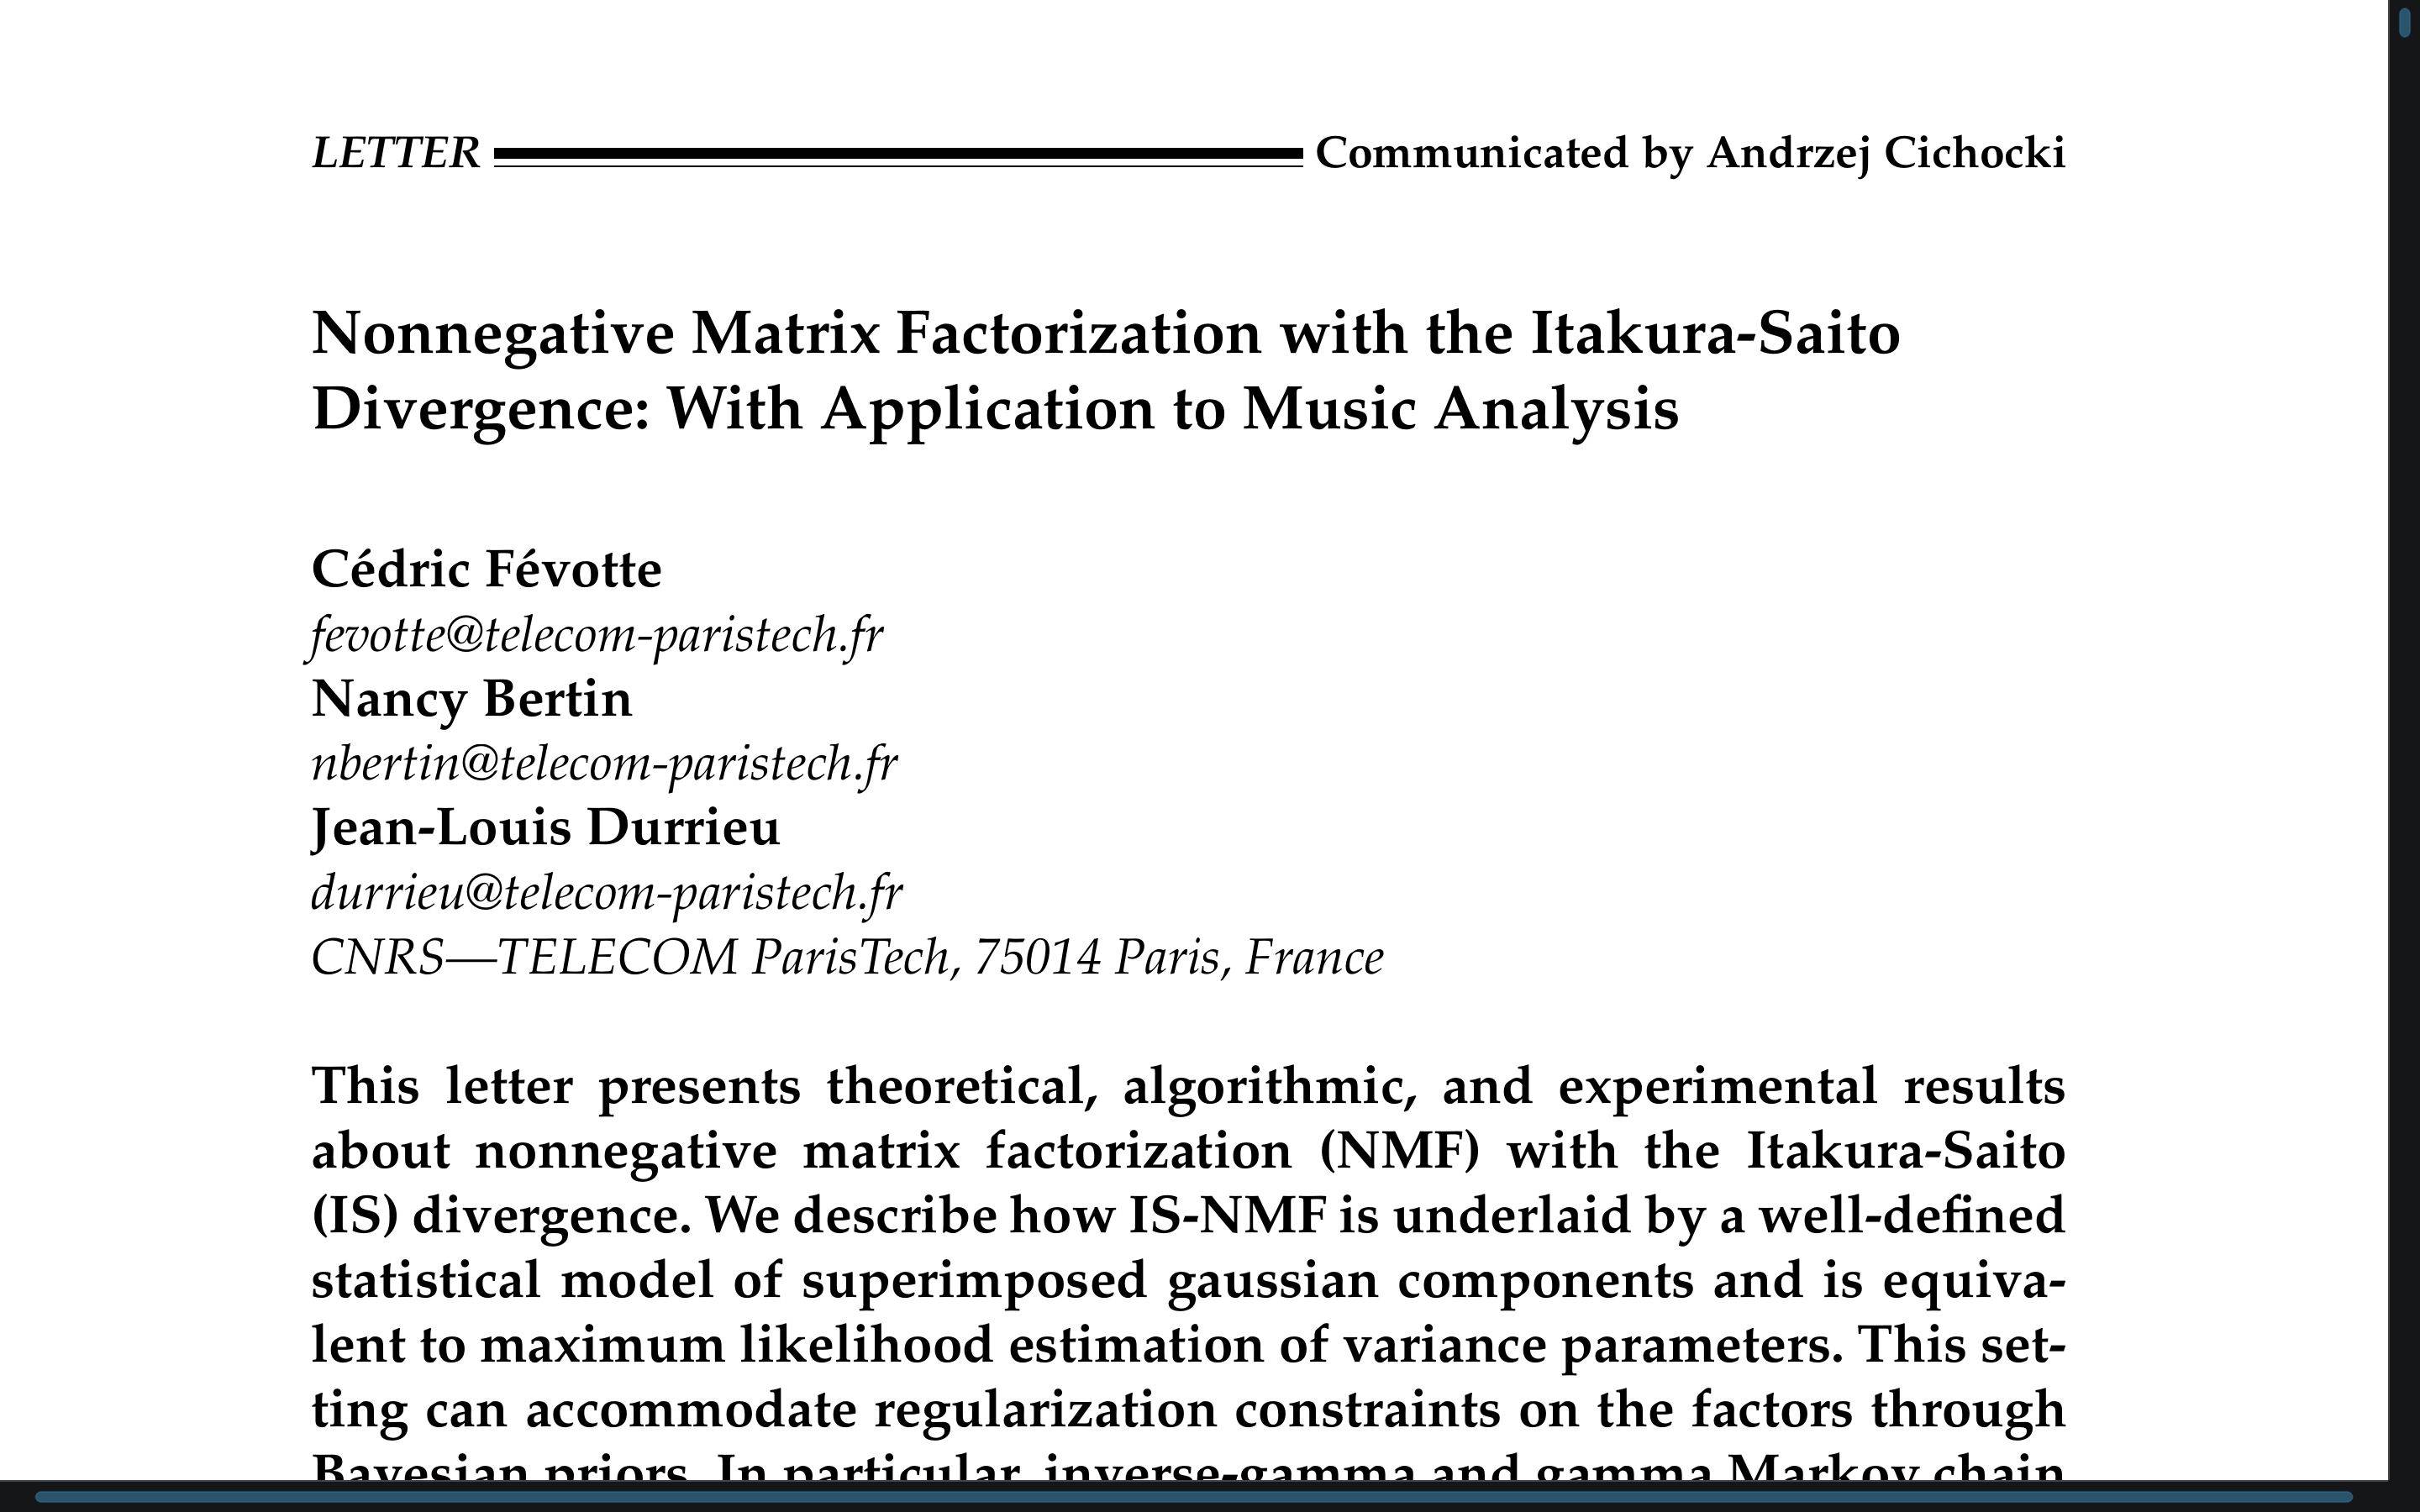
\includegraphics[width=\textwidth]{images/Screenshot_20260321_122109.png}
    \end{minipage}
    \hfill
    \begin{minipage}{0.30\textwidth}
      \centering
      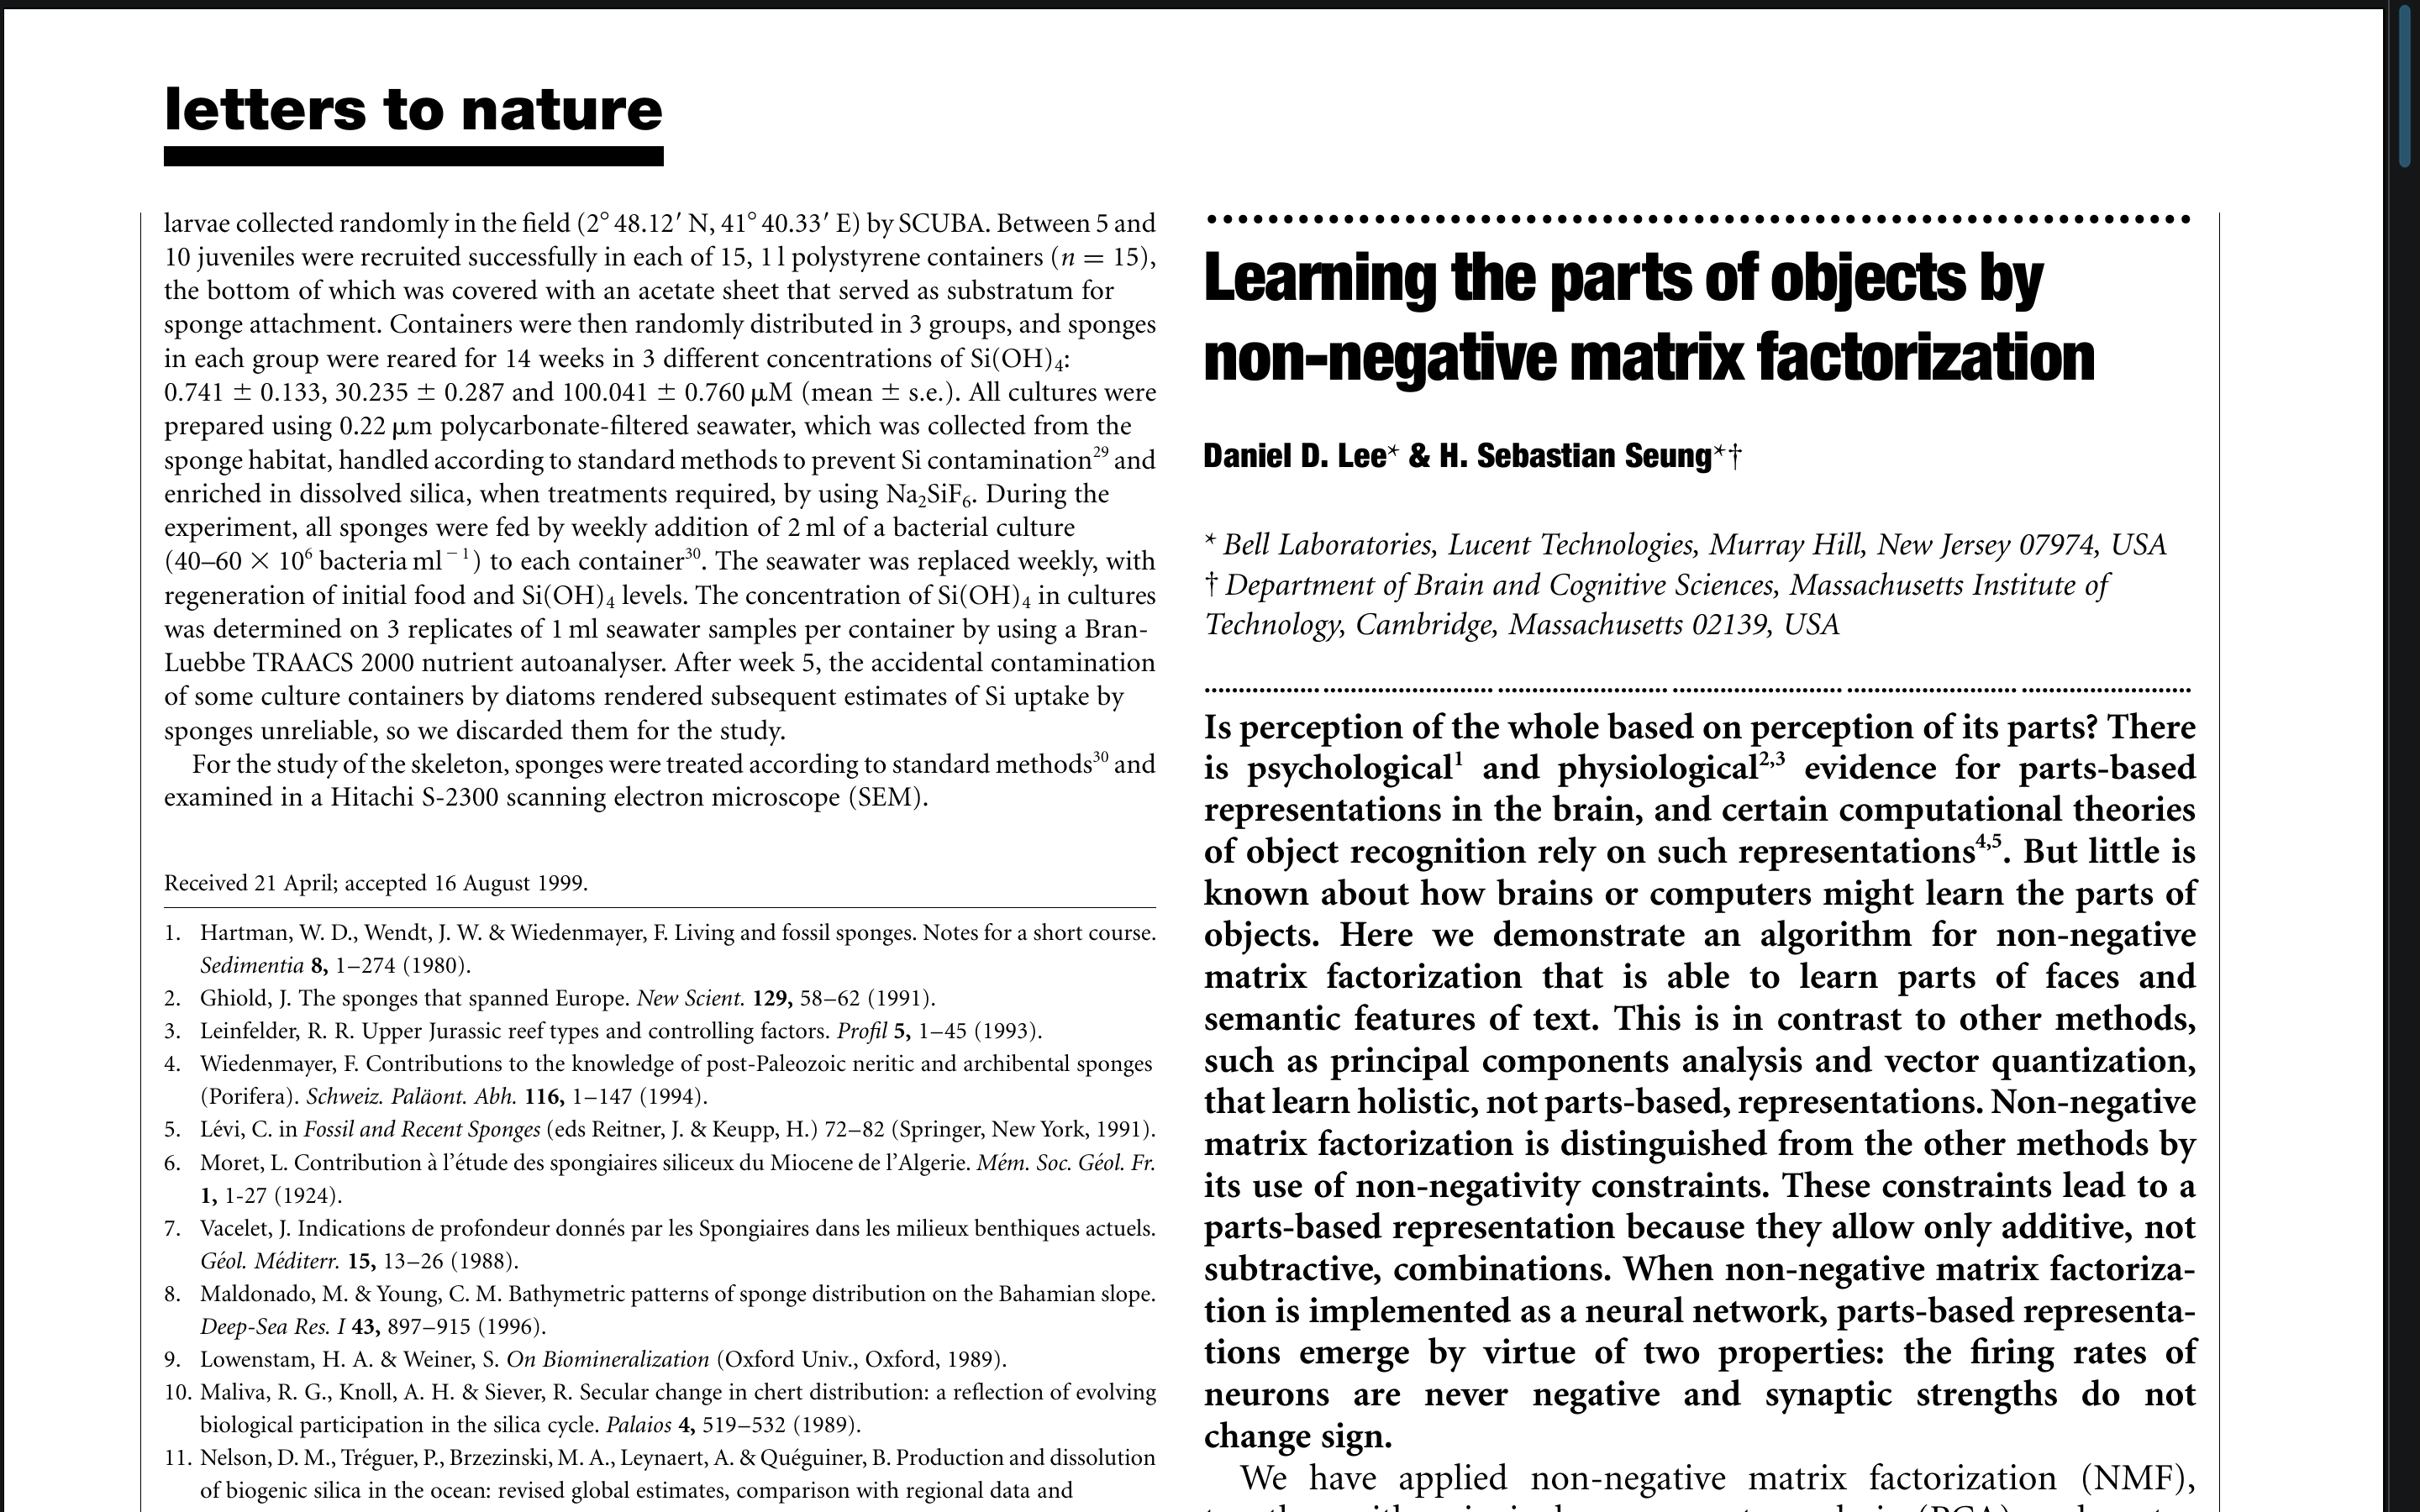
\includegraphics[width=\textwidth]{images/Screenshot_20260321_123139.png}
    \end{minipage}
    \hfill
    \begin{minipage}{0.30\textwidth}
      \centering
      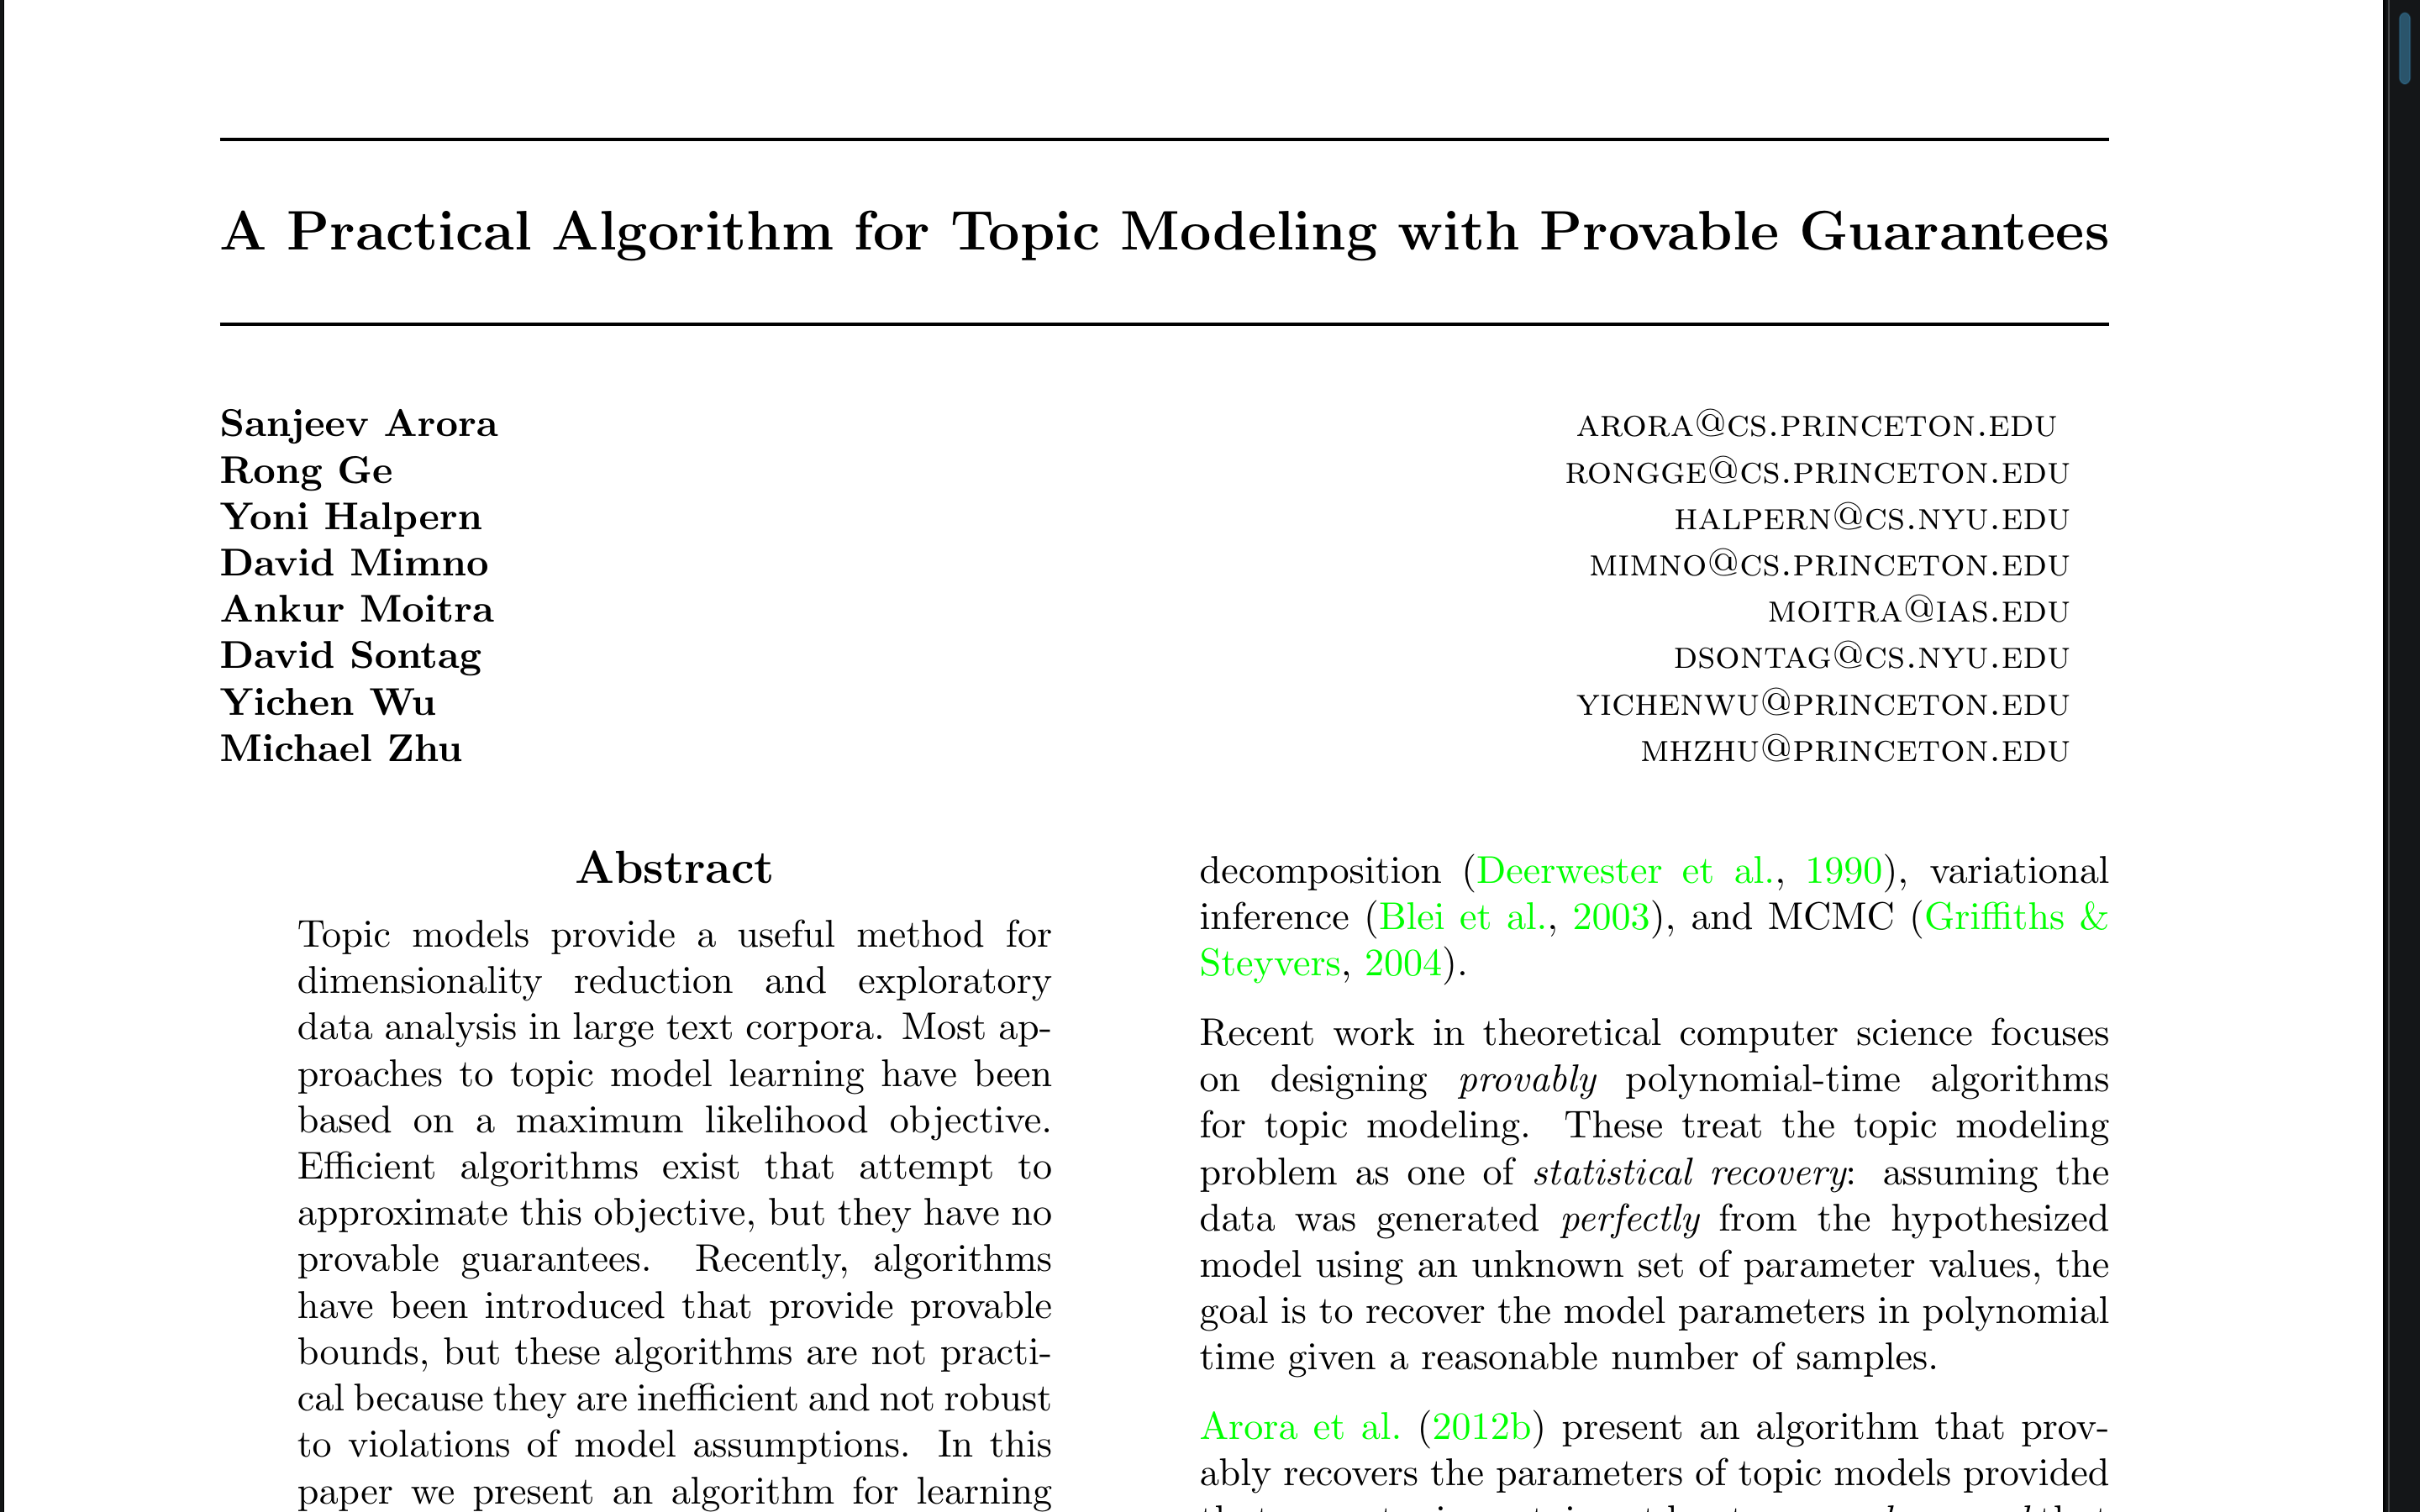
\includegraphics[width=\textwidth]{images/Screenshot_20260322_143749.png}
    \end{minipage}
  \end{figure}
  \end{frame}


  \begin{frame}{Example: learning parts of objects with NMF \small{(Lee \& Seung \cite{lee1999})}}
    \begin{columns}
      \column{0.5\textwidth}
      \begin{figure}
        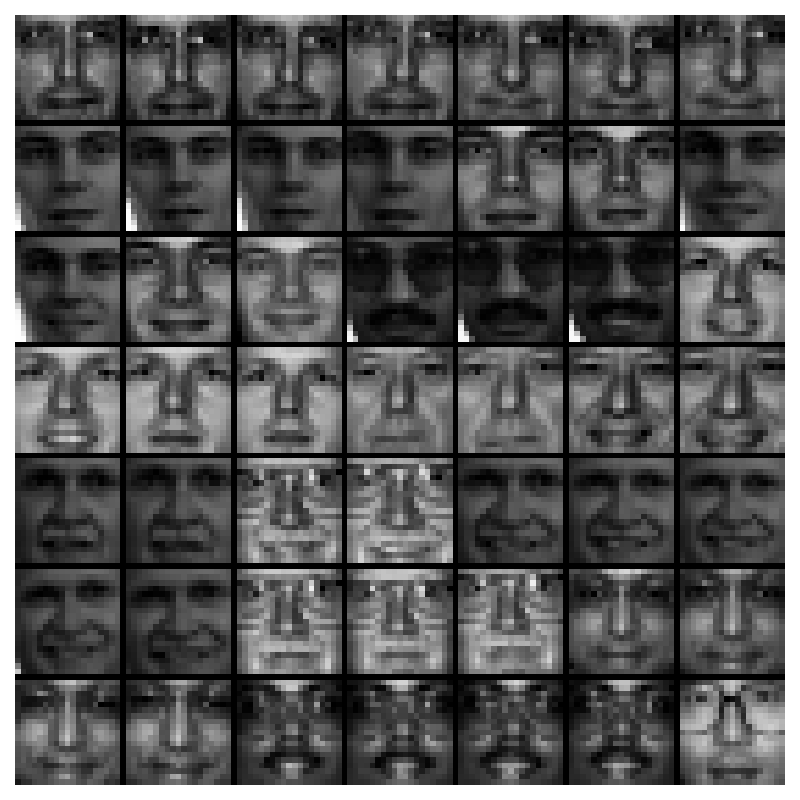
\includegraphics[width=0.5\textwidth]{../Imgs/CBCL_Original.png}
        \caption{\tiny{Sample images from the CBCL face dataset.}}
        \label{CBCL original}
        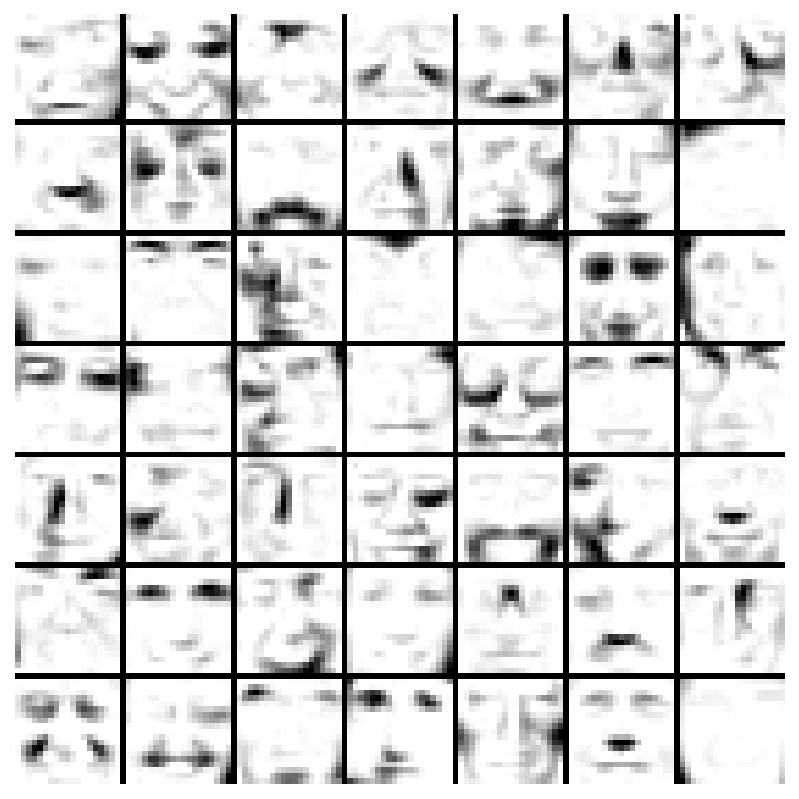
\includegraphics[width=0.5\textwidth]{../Imgs/Basis images.png}
        \caption{\tiny{Basis images obtained from NMF.}}
        \label{CBCL basis NMF}
      \end{figure}
      
      \column{0.5\textwidth}
      \begin{itemize}
        \item CBCL face dataset $\rightarrow$ 2429 images of faces with 19x19 pixels.
        \item NMF with $r = 49$ $\rightarrow$ 49 basis images and corresponding coefficients.
        \item Basis images extract \alert{facial features}.
        \item Columns of $H$ contain the weight of each feature for each image.
        \item Original images reconstructed as $V[:,i] \approx \sum_{k=1}^r W[:,k] H[k,i]$.
      \end{itemize}
    \end{columns}
  \end{frame}

\section{Algorithms}

\subsection{MU}

\begin{frame}{Lee and Seung proposed the Multiplicative Updates (MU).}
\textbf{Can be interpreted as a scaled \alert{gradient descent} method:}

the gradient of the cost function with respect to $H$ is given by:
\begin{equation}
\nabla_H\frac{1}{2}\|V - WH\|_F^2 = W^TWH - W^TV
\end{equation}
taking a step of size:
\begin{equation}
  \eta_k = \frac{H}{W^TWH}
\end{equation}
yields the multiplicative update rule:
\begin{block}{MU for $H$}
\begin{equation}
H \leftarrow H \circ \frac{W^TV}{W^TWH}
\end{equation}
\end{block}
\end{frame}

\begin{frame}{Multiplicative Updates (MU) for NMF}
  \begin{block}{}
  \begin{algorithm}[H]
    \caption{Multiplicative Update for NMF}
    \label{MU}
    \begin{algorithmic}
        \Require \( V \in \mathbb{R}_+^{m \times n} \), rank \( r \), initial factors \( W^{(0)} \in \mathbb{R}_+^{m \times r} \), \( H^{(0)} \in \mathbb{R}_+^{r \times n} \)
        \While{stopping criterion not met}
            \State \( H^{(k+1)} \leftarrow H^{(k)} \circ \frac{W^{(k) \top} V}{W^{(k) \top} W^{(k)} H^{(k)}} \)
            \Comment{Update for H}
            \State \( W^{(k+1)} \leftarrow W^{(k)} \circ \frac{V H^{(k+1) \top}}{W^{(k)} H^{(k+1)} H^{(k+1) \top}} \)
            \Comment{Update for W}
            \EndWhile
        \State \Return \( W, H \)
    \end{algorithmic}
\end{algorithm}
\end{block}
\end{frame}

\subsection{PGD}

\begin{frame}{Projected Gradient Descent (PGD) for NMF}
  \begin{block}{}
  \begin{algorithm}[H]
    \caption{Projected Gradient Descent for NMF}
    \label{Projected Gradient}
    \begin{algorithmic}[1] 
        \Require \( V \in \mathbb{R}_+^{m \times n} \), rank \( r \), initial factors \( W^{(0)} \in \mathbb{R}_+^{m \times r} \), \( H^{(0)} \in \mathbb{R}_+^{r \times n} \)
        % \output \( W \in \mathbb{R}_+^{m \times r} \), \( H \in \R_+^{r \times n} \) such that \( V \approx WH \)
        \While{stopping criterion not met}
            \State LW \( \leftarrow \|W^{(k)}\|_2^2 \)
            \State LH \( \leftarrow \|H^{(k)}\|_2^2 \)
            \Comment{Lipschitz constants}
            \State Grad\_W \( \leftarrow W^{(k)} H^{(k)} H^{(k) \top} - V H^{(k) \top} \)
            \Comment{Gradient w.r.t. W}
            \State $W^{(k+1)}$ \( \leftarrow \max\left(0, W^{(k)} - \frac{1}{LW} \text{Grad\_W} \right) \)
            \Comment{Update for W}
            \State Grad\_H \( \leftarrow W^{(k+1) \top} W^{(k+1)} H^{(k)} - W^{(k+1) \top} V \)
            \Comment{Gradient w.r.t. H}
            \State $H^{(k+1)} \leftarrow \max\left(0, H^{(k)} - \frac{1}{LH} \text{Grad\_H} \right)$
            \Comment{Update for H}
        \EndWhile
        \State \Return \( W, H \)
    \end{algorithmic}
\end{algorithm}
\end{block}  
\end{frame}

\subsection{ALS}

\begin{frame}{Alternating Least Squares (ALS) for NMF}
  \begin{block}{}
    \begin{algorithm}[H]
    \caption{Alternating Least Squares for NMF}
    \label{ALS}
    \begin{algorithmic}
        \Require \( V \in \mathbb{R}_+^{m \times n} \), rank \( r \), initial factors \( W^{(0)} \in \mathbb{R}_+^{m \times r} \), \( H^{(0)} \
\in \mathbb{R}_+^{r \times n} \)
        % \output \( W \in \mathbb{R}_+^{m \times r} \), \( H \in \R_+^{r \times n} \) such that \( V \approx WH \)
        \While{stopping criterion not met}
            \For{i = 1 to m}\Comment{m independent linear least squares}
                \State \( W(i,:) \leftarrow \max\left(0, \arg\min_{w} \|V(i,:) - w H^{(k)}\|_2^2 \right) \)
                
            \EndFor
            \For{j = 1 to n} \Comment{n independent linear least squares}
                \State \( H(:,j) \leftarrow \max\left(0, \arg\min_{h} \|V(:,j) - W^{(k)}h\|_2^2 \right) \)
            \EndFor
            % \State \( W^{(k + 1)} \leftarrow \max\left(0, \arg\min_W \|V - WH^{(k)}\|_F^2  \right) \)
            % \State \( H^{(k + 1)} \leftarrow \max\left(0, \arg\min_H \|V -  W^{(k + 1)}H\|_F^2  \right) \)
        \EndWhile
        \State \Return \( W, H \)
    \end{algorithmic}
\end{algorithm}
  \end{block}
\end{frame}

\subsection{HALS}

\begin{frame}{Hierarchical Alternating Least Squares (HALS) for NMF}
  \begin{block}{}
  \begin{algorithm}[H]
    \caption{Hierarchical Alternating Least Squares for NMF}
    \label{HALS}
    \begin{algorithmic}[1]
        \Require \( V \in \mathbb{R}_+^{m \times n} \), rank \( r \), initial factors \( W^{(0)} \in \mathbb{R}_+^{m \times r} \), \( H^{(0)} \in \mathbb{R}_+^{r \times n} \)
        \While{stopping criterion not met}
            \For{\( \ell = 1 \) to \( r \)}
                \State \( \tilde{R}_{\ell} \leftarrow V - \sum_{k\not=\ell}W[:,k]H[k,:] \)
                \Comment{Residual matrix w.r.t. \(\ell\)}
                \State \( H[\ell,:] \leftarrow \max\left(0, \frac{\tilde{R}_{\ell}^\top W[:,\ell]}{W[:,\ell]^\top W[:,\ell]} \right) \)
                            
                \EndFor
            \For{\( \ell = 1 \) to \( r \)}
                \State \( \tilde{R}_{\ell} \leftarrow V - \sum_{k\not=\ell}W[:,k]H[k,:] \)
                \State \( W[:,\ell] \leftarrow \max\left(0, \frac{\tilde{R}_{\ell} H[\ell,:]^\top}{H[\ell,:] H[\ell,:]^\top} \right) \)
            \EndFor
        \EndWhile
        \State \Return \( W, H \)
    \end{algorithmic}
\end{algorithm}
  \end{block}
\end{frame}

\section{Implementation and Results}

\subsection{Python implementation}

\begin{frame}{The Algorithms have been implemenetd in Python}
  \begin{figure}
    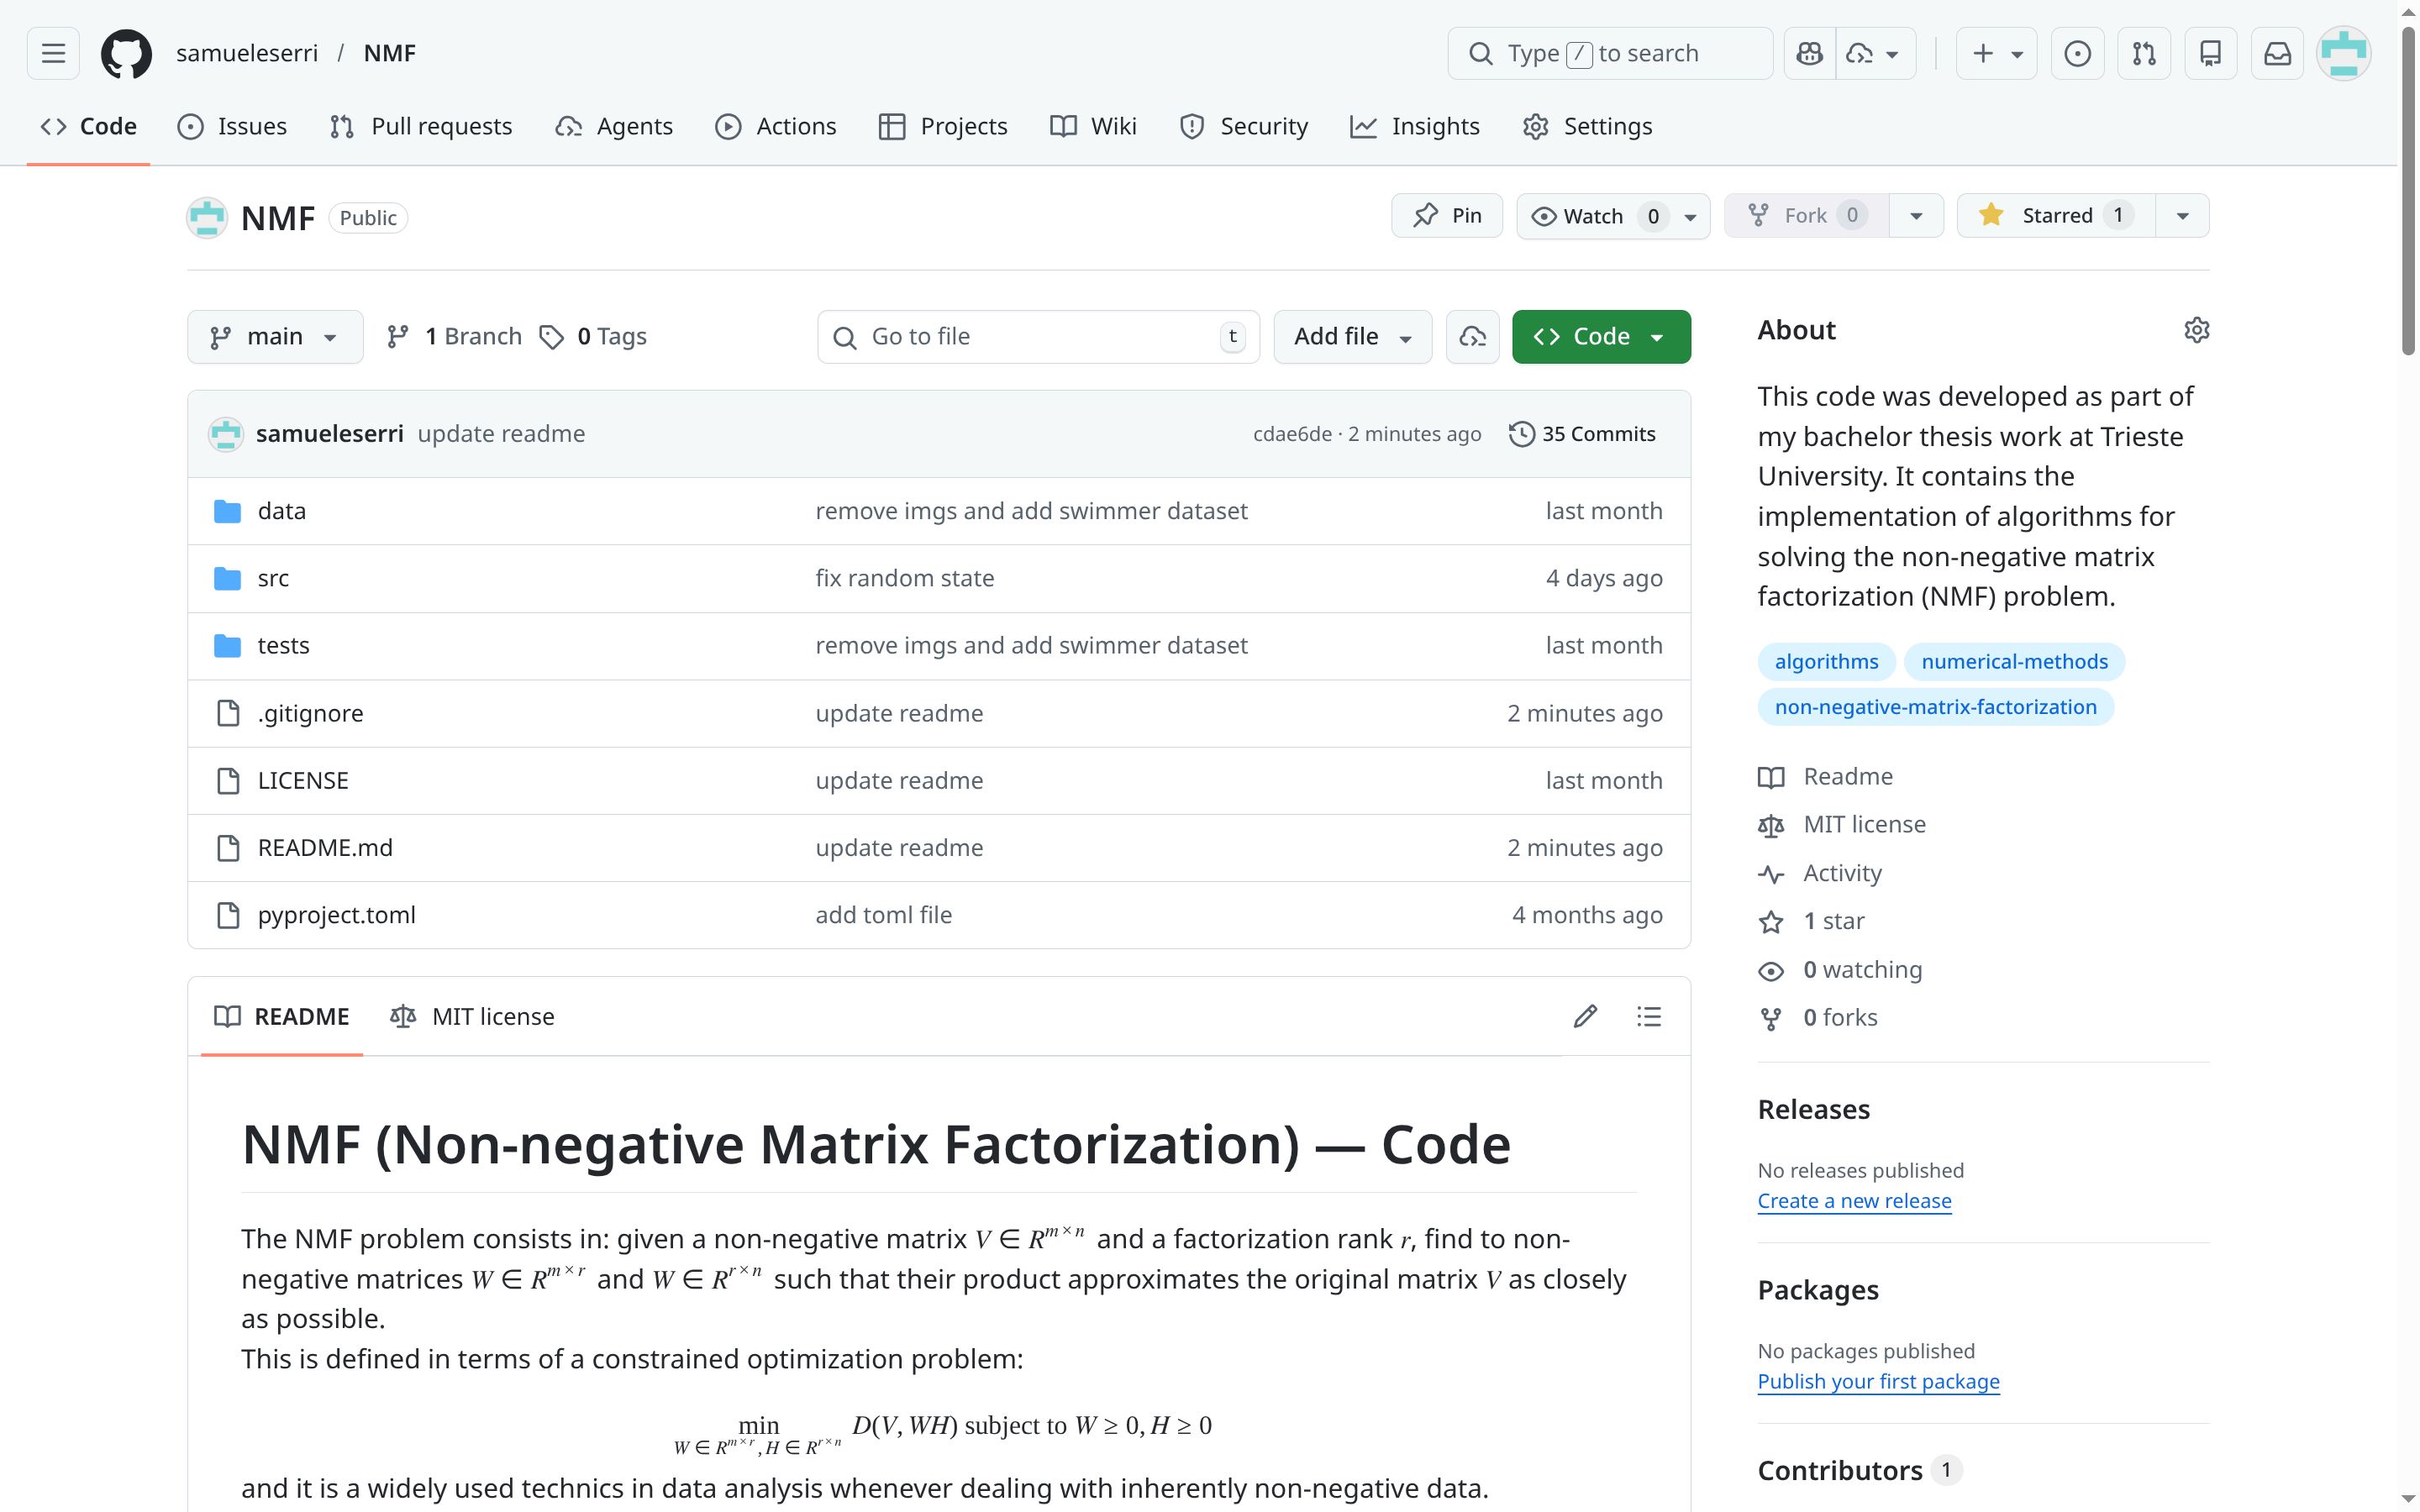
\includegraphics[width=1\textwidth]{images/Screenshot_20260322_114228.png}
      \caption{\url{https://github.com/samueleserri/NMF.git}}    
  \end{figure}
\end{frame}

\subsection{Numerical simulations}

\begin{frame}{Make Titles Informative.}
  \begin{columns}
    \column{0.5\textwidth}
    \begin{figure}
      
\includegraphics[width=1\textwidth]{images/CBCL_random_init.png}
      \caption{\tiny{Average relative reconstruction error for each algorithm averaged over 10 random initializations on the CBCL dataset.}}
    \end{figure}
    
    \begin{table}[htbp]
      \centering
      \tiny
      \begin{tabular}{|l|l|l|}
        \hline
        Algorithm & Avg. iterations & Avg. time/iter (s) \\ \hline
        MU        & 324             & $9.26 \times 10^{-2}$ \\ \hline
        HALS      & 362             & $8.29 \times 10^{-2}$ \\ \hline
        ALS       & 144             & $2.08 \times 10^{-1}$ \\ \hline
        PGD       & 282             & $1.06 \times 10^{-1}$ \\ \hline
      \end{tabular}
      \caption{\tiny{Average iterations and time per iteration for each algorithm.}}
      \label{tab:CBCL results 49}
    \end{table}
    
    \column{0.5\textwidth}
    \begin{block}{\small }
      \tiny
      Numerical simulations on the CBCL face dataset with rank $r = 49$, averaged over 10 random initialization.
      Each algorithm was run for 30 seconds, and the average number of iterations and time per iteration were recorded.
    \end{block}
    
    \vspace{1 cm}
    
    \begin{block}{\small Results}
      \tiny
      HALS converges the fastest and reaches the lowest relative reconstruction error within the 30 seconds.
      ALS perform the worst, with the highest time per iteration and lowest number of iterations.
      PGD has a higher time per iteration than MU and HALS, but converges faster than ALS.
      MU and PGD have similar performance.

    \end{block}
  \end{columns}
\end{frame}


% All of the following is optional and typically not needed. 
\appendix
\section<presentation>*{\appendixname}
\subsection<presentation>*{For Further Reading}

\begin{frame}[allowframebreaks]
  \frametitle<presentation>{For Further Reading and References}
    
  \begin{thebibliography}{10}
    
  \beamertemplatebookbibitems
  % Start with overview books.

  \bibitem{gillis2020nonnegative}
    Gillis, Nicolas.
    \newblock {\em Nonnegative matrix factorization}.
    \newblock SIAM, 2020.
 
    
  \beamertemplatearticlebibitems
  % Followed by interesting articles. Keep the list short. 

  \bibitem{lee1999}
    Lee, D.D. and Seung, H.S.
    \newblock Learning the parts of objects by non-negative matrix factorization.
    \newblock {\em Nature},
    1999.
  \end{thebibliography}
  
  \vspace*{0.5cm}
  
  \begin{center}
    \textbf{Thank you for your attention!}
  \end{center}
\end{frame}

\end{document}